% Numbers come from artifacts/reported_results/2026-10-04-rollout-fidelity/ (see its README).
% Generated by artifacts/reported_results/2026-10-04-rollout-fidelity/generate.py; do not edit.
\newcommand{\RFMainGenerate}{49.2}
\newcommand{\RFFixGenerate}{36.8}
\newcommand{\RFCanvasGenerate}{36.5}
\newcommand{\RFPackGenerate}{28.4}
\newcommand{\RFFixSaving}{25\%}
\newcommand{\RFPackSaving}{22\%}
\newcommand{\RFTotalSaving}{42\%}
\newcommand{\RFMainReward}{2.80}
\newcommand{\RFFixReward}{4.62}
\newcommand{\RFPostFixRewardMin}{4.45}
\newcommand{\RFPostFixRewardMax}{4.77}
\newcommand{\RFLongTailRollout}{2}
\newcommand{\RFWorkerKv}{5,938}
\newcommand{\RFTrainerKv}{2,263}
\newcommand{\RFRatioBuggy}{5.0}
\newcommand{\RFRatioHealthy}{3.4}
\newcommand{\RFRatioHealthyEdit}{5.4}
\newcommand{\RFTailMin}{1.16}
\newcommand{\RFTailMax}{1.84}
\newcommand{\RFSmallBase}{99.3}
\newcommand{\RFSmallOverlap}{93.7}
\newcommand{\RFSmallSteal}{77.4}
\newcommand{\RFSmallBoth}{71.5}
\newcommand{\RFSmallBothSaving}{28\%}
\newcommand{\RFLargeBase}{128.4}
\newcommand{\RFLargeSteal}{131.1}
\newcommand{\RFLargeFirstBase}{118.3}
\newcommand{\RFLargeFirstSteal}{131.5}
\newcommand{\RFLargeStealNoOverlap}{132.2}
\newcommand{\RFLargeFirstStealNoOverlap}{133.3}
\newcommand{\RFSmallFirstStepSteal}{2.7}
\newcommand{\RFTrainSlowSteadyMin}{1}
\newcommand{\RFTrainSlowSteadyMax}{5}
\newcommand{\RFTrainSlowFirstMin}{3}
\newcommand{\RFTrainSlowFirstMax}{12}
\newcommand{\RFTrainSlowOwnerMin}{2}
\newcommand{\RFTrainSlowOwnerMax}{3}
\newcommand{\RFLargeTail}{90.8}
\newcommand{\RFLargeTailSteal}{68.4}
\newcommand{\RFTtoiBase}{150.2}
\newcommand{\RFTtoiBalanced}{108.6}
\newcommand{\RFTtoiIdle}{29\%}
\newcommand{\RFNaiveBalanced}{133.9}
\newcommand{\RFNaiveSteal}{115.9}
\newcommand{\RFNaiveGap}{25}
\newcommand{\RFStealRecovered}{18}
\newcommand{\RFStealPixelsEditMax}{2}
\newcommand{\RFPackedGroupEight}{13.96}
\newcommand{\RFUnpackedGroupEight}{18.04}


\section{Case Study II: Rollout Fidelity and Request Shaping}
\label{sec:fidelity}

Whereas Section~\ref{sec:reward} examined how generated trajectories are scored, this case study examines the boundary between the trajectory IR and an external rollout engine.
Two properties at the engine boundary govern whether optimization updates match the scored behavior and how efficiently rollouts execute: first, the rollout engine and the training backend must condition on identical context representations; second, requests sent to the engine should pack sibling samples under a shared prompt so that prompt conditioning is encoded once per group rather than once per sample.
Because a rollout adapter returns a structurally well-formed \sample{} regardless of how the engine internally constructs its conditioning or batches requests, verifying these properties requires explicit checks and request-shaping contracts across the engine boundary.

\paragraph{Source scope.}
This case study examines four stacked changes to the vLLM-Omni BAGEL rollout path proposed in UniRL pull requests~\#547--\#550 (open at the time of writing), affecting both text-to-image (\texttt{t2i}) and instruction-guided image-to-image editing (\texttt{it2i}) workloads.
All measurements below were collected on a single node of eight NVIDIA H20 GPUs, with per-run records and table generators archived under \codepath{artifacts/reported\_results/2026-10-04-rollout-fidelity/}.
The dynamic load-balancing prototype evaluated in Section~\ref{sec:fidelity-tail} was measured on an experimental branch without an open pull request.

\subsection{Conditioning Mismatch Undetected by the Importance Ratio}
\label{sec:fidelity-layout}

In instruction-guided image editing (\texttt{it2i}), the policy conditions on a source image alongside the edit instruction.
To guarantee rollout--replay consistency, UniRL constructs this conditioning on the worker---applying its own image transforms and vision encoder---and injects the resulting key--value contexts directly into the vLLM-Omni serving engine so that the trainer replays against identical contexts during optimization.
Following an upstream serving-engine migration, however, three helper functions in the BAGEL pipeline continued to read the injected conditioning field from the outer request-batch wrapper after the caller had already unwrapped it to an individual request object.
Because the looked-up attribute was absent on the unwrapped object, the injected contexts were silently ignored, and the serving engine fell back to its internal image-to-image preprocessing path---using a different image transform at a fixed resolution, a sampled rather than mean latent encoding, and an output canvas sized to the source image rather than the recipe target.

Despite this bug, training completed without raising an error: every image-editing rollout generated samples under the engine's fallback conditioning (\RFWorkerKv{} context tokens) and replayed them under the trainer's conditioning (\RFTrainerKv{} context tokens at the same $512\times512$ source resolution).
Notably, standard importance-ratio monitoring did not flag the discrepancy.
Before the first optimizer update of a rollout, the current policy $\theta$ equals the behavior policy $\pi_v$, so the importance ratio $\rho$ against the rollout behavior anchor should equal 1 up to floating-point noise.
In practice, the observed ratio remained close to 1 despite the mismatch: the maximum first-update deviation $|\rho - 1|$ was $\RFRatioBuggy\times10^{-5}$ with the conditioning bug versus $\RFRatioHealthy\times10^{-5}$ after the fix, well within the $\RFRatioHealthyEdit\times10^{-5}$ deviation observed in healthy image-editing runs (Table~\ref{tab:fidelity-layout}).
This insensitivity arises from how denoising transition log probabilities are reduced.
Both the rollout engine and the trainer compute the Gaussian log-density of each denoising transition by averaging over all latent elements rather than summing across them; consequently, a perturbation to the predicted velocity mean---even one large enough to alter the generated image---is divided by the number of latent dimensions (tens of thousands of elements at $512\times512$ resolution) before entering the log-probability ratio.
Under element-mean reduction, the importance ratio cannot distinguish a structural conditioning mismatch from benign numerical noise.
Moreover, when a recipe uses the trainer-recomputed replay anchor (the default in several diffusion configurations), the baseline log probabilities are recomputed on the trainer itself, making the first-update ratio identically 1 by construction.

To detect such discrepancies directly, UniRL adds a structural token-layout check across the rollout--replay boundary (UniRL pull request~\#548).
The engine hook that injects initial noise now also records three integers and the output canvas dimensions---the generation context token length, its positional offset, and the rendered height and width---which are returned through the capture channel into the trajectory's model conditions $C_i$ and compared row-by-row against the context reconstructed by the trainer during replay.
Any discrepancy raises an exception on the first replay pass and logs both layouts.
Because the trainer already constructs the replay context, the check adds zero tensor-compute overhead; conditioning paths that carry pre- materialized contexts bypass the check.
Table~\ref{tab:fidelity-layout} summarizes the validation probes caught by this check.
The importance-ratio check is retained as an optional secondary diagnostic for detecting weight-publication desynchronization or mismatched LoRA adapters, where the model weights themselves differ between rollout and replay.

\begin{table}[H]
\caption{Validation probes for the structural token-layout check across text-to-image (\texttt{t2i}) and image-to-image editing (\texttt{it2i}) paths. ``Engine'' and ``Trainer'' columns report the generation-context token counts on each side. The final column reports the maximum first-update importance-ratio deviation $|\rho-1|$ in the same run.}
\label{tab:fidelity-layout}
\centering
\small
% Generated by artifacts/reported_results/2026-10-04-rollout-fidelity/generate.py; do not edit.
\begin{tabularx}{\textwidth}{@{}Xlrrll@{}}
\toprule
Probe & Path & Engine & Trainer & Layout check & $|\rho-1|$ \\
\midrule
Main before the injection fix & it2i & 5,938 & 2,263 & raises at the first replay & $5.0\times10^{-5}$ \\
Trainer prompt lengthened by three tokens & t2i & 63 & 66 & raises at the first replay & -- \\
Trainer source image halved in width & it2i & 2,268 & 1,161 & raises at the first replay & -- \\
After the injection fix & it2i & 2,263 & 2,263 & passes & $3.4\times10^{-5}$ \\
Healthy run (rollout anchor) & t2i & equal & equal & passes & $8.6\times10^{-6}$ \\
Healthy run (rollout anchor) & it2i & equal & equal & passes & $5.4\times10^{-5}$ \\
Healthy run (replay anchor) & it2i & equal & equal & passes & $0$ \\
\bottomrule
\end{tabularx}

\end{table}

Restoring the injected conditioning (UniRL pull request~\#547) affected both rollout latency and initial judge scores.
Generation time for 16 edits per rank decreased from \RFMainGenerate{}\,s to \RFFixGenerate{}\,s (\RFFixSaving{}), because the engine's fallback path encoded the source image into nearly four times as many vision tokens as UniRL's encoder path (\RFWorkerKv{} versus \RFTrainerKv{} total context tokens).
Simultaneously, the mean EditScore reward on the first rollout---evaluated on identical prompts prior to any optimizer update---increased from \RFMainReward{} to \RFFixReward{} (Figure~\ref{fig:fidelity-chain}), reflecting the quality difference between the two conditioning representations on the pretrained checkpoint.

\subsection{Per-Group Output Canvas Resolution}
\label{sec:fidelity-canvas}

Previously, every rollout batch required a single uniform output resolution fixed by the recipe, because the trajectory's latent segment stores latents as a single dense tensor and the rollout adapter passed a single canvas size to the engine.
Production prompt datasets, however, contain prompts with varying target aspect ratios and resolutions; forcing a single resolution either wastes compute on low-resolution prompts or truncates high-resolution ones.

UniRL pull request~\#549 allows each dataset example to specify its own target canvas dimensions in its metadata $M_0$.
During rollout, the trajectory resolves the target canvas for each frontier row from its root ancestor (falling back to the recipe default), and the rollout adapter dispatches one engine call per contiguous run of rows sharing the same canvas size.
To keep the latent segment tensor dense across a mixed-resolution batch, smaller canvases are right-padded along the token dimension to match the recipe's maximum canvas size, and the trainer slices each row back to its true token count during replay; canvases exceeding the recipe maximum are rejected at admission.
Because all sibling samples forked from a root prompt share the same canvas, group-relative credit assignment, the micro-batched \texttt{RewardStack} of Section~\ref{sec:reward-overlap}, and downstream scorers require no modification.
Datasets without per-example canvas metadata execute identically to the fixed-resolution path.
Rollout backends that support only a single resolution per batch---including the train-side diffusion adapter, non-BAGEL serving adapters, and video pipelines---explicitly reject the per-row canvas metadata field rather than silently rendering at the default resolution.

This padding scheme applies to objectives whose replay anchor stores a single scalar per denoising transition (such as Flow-GRPO).
Objectives that store per-token replay anchors or consume the dense latent field directly still require a uniform canvas across the batch and now fail fast with a descriptive error when given mixed-canvas inputs.

\begin{table}[H]
\caption{Generation time (seconds) for one prompt group of four sibling samples across three output canvas resolutions on a single H20 rank, for image-to-image editing (\texttt{it2i}, which additionally encodes a $512\times512$ source image) and text-to-image generation (\texttt{t2i}). The $768\times768$ \texttt{t2i} entry was measured on an earlier commit of the same branch.}
\label{tab:fidelity-canvas}
\centering
\small
% Generated by artifacts/reported_results/2026-10-04-rollout-fidelity/generate.py; do not edit.
\begin{tabular}{@{}lrrrr@{}}
\toprule
Canvas & Image tokens & it2i, one per sample & it2i, packed & t2i, packed \\
\midrule
$512\times512$ & 1,024 & 9.05 & 7.25 & 6.50 \\
$768\times768$ & 2,304 & 17.45 & 15.76 & 14.55 \\
$1{,}024\times1{,}024$ & 4,096 & 30.48 & 28.83 & 27.00 \\
\bottomrule
\end{tabular}

\end{table}

Table~\ref{tab:fidelity-canvas} shows that generation latency scales approximately linearly with the number of image tokens, creating a $4\times$ cost difference between $512\times512$ and $1{,}024\times1{,}024$ canvases within the same batch.
When each data-parallel rank receives two prompt groups drawn in dataset order from a mixed-resolution prompt set, the slowest rank requires \RFTailMin{}--\RFTailMax{}$\times$ the mean per-rank generation time, and the synchronous rollout barrier forces all other ranks to wait.

\subsection{Sibling Request Packing for Image Editing}
\label{sec:fidelity-pack}

Group-relative credit assignment generates multiple sibling samples per prompt.
In the original BAGEL image-editing adapter, each sibling sample was dispatched as an independent engine request, causing the engine to recompute the same vision-encoder passes and key--value conditioning contexts for every sibling in the group.
With sibling request packing (UniRL pull request~\#550), when guidance scales permit, the adapter consolidates contiguous sibling rows from the same prompt group into a single engine request; the engine encodes the source conditioning once and broadcasts the resulting context across all siblings in the group.
At 16 edits per rank ($512\times512$), packing reduces per-rank generation time from \RFCanvasGenerate{}\,s to \RFPackGenerate{}\,s (\RFPackSaving{}, Table~\ref{tab:fidelity-chain}) at the cost of roughly 2\,GiB of additional peak GPU memory, while a single group of eight siblings drops from \RFUnpackedGroupEight{}\,s to \RFPackedGroupEight{}\,s.
The text-to-image path already packed sibling requests and is unaffected.

Because initial noise tensors are indexed per row, a packed request can span any contiguous subset of a sibling group rather than requiring the full group at once.
Consequently, the adapter no longer requires \texttt{RewardStack} (Section~\ref{sec:reward-overlap}) to round micro-batch sizes up to full group boundaries: a four-row micro-batch from an eight-sibling group executes as a single four-sample packed request.

\subsection{Combined Effect of the Four Changes}
\label{sec:fidelity-combined}

\begin{figure}[H]
\centering
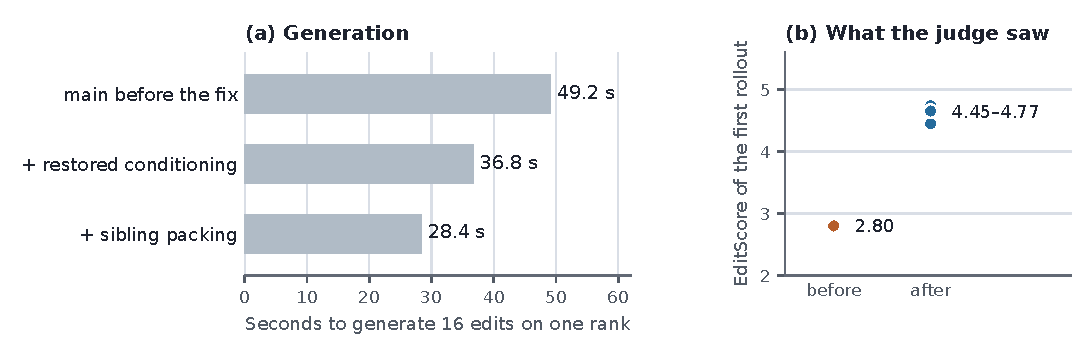
\includegraphics[width=\textwidth]{artifacts/reported_results/2026-10-04-rollout-fidelity/figures/rollout_chain.pdf}
\caption{Cumulative effect of the four rollout-fidelity changes on BAGEL image editing (\texttt{it2i}) on one eight-GPU H20 node with a remote EditScore 8B judge. Left: per-rank generation time for 16 edits. Right: mean judge score on the first rollout prior to any optimizer step; points after the fix represent independent runs on the same initial prompt batch.}
\label{fig:fidelity-chain}
\end{figure}

\begin{table}[H]
\caption{Cumulative ablation of the four rollout-fidelity changes on BAGEL image-to-image editing (\texttt{it2i}) with LoRA on one eight-GPU H20 node (vLLM-Omni rollout, 16 prompts $\times$ 8 samples at $512\times512$, remote EditScore 8B judge). ``Generation'' reports the slowest rank's generation time for its 16 rows; ``First-rollout reward'' reports the mean judge score before the first optimizer update.}
\label{tab:fidelity-chain}
\centering
\small
% Generated by artifacts/reported_results/2026-10-04-rollout-fidelity/generate.py; do not edit.
\begin{tabularx}{\textwidth}{@{}Xrrrr@{}}
\toprule
Rollout path & Rollouts & Generation (s) & vs.\ \texttt{main} & First-rollout reward \\
\midrule
\texttt{main} before the fix & 1 & 49.2 & -- & 2.80 \\
+ restored it2i conditioning (\#547) & 1 & 36.8 & $-$25\% & 4.62 \\
+ per-group canvas (\#549) & 1 & 36.5 & $-$26\% & 4.77 \\
+ sibling packing (\#550) & 4 & 28.4 & $-$42\% & 4.45--4.74 \\
\bottomrule
\end{tabularx}

\end{table}

Table~\ref{tab:fidelity-chain} and Figure~\ref{fig:fidelity-chain} summarize the cumulative impact of UniRL pull requests~\#547--\#550 on the $512\times512$ image-editing workload: per-rank generation time drops by \RFTotalSaving{} (from \RFMainGenerate{}\,s to \RFPackGenerate{}\,s), while the first-rollout EditScore mean increases from \RFMainReward{} to \RFPostFixRewardMin{}--\RFPostFixRewardMax{}.
Across all arms, the first-update importance ratio remains within $10^{-4}$ of 1, and the structural token-layout check (enabled from \#548 onward) passes on every replay, including configurations where \texttt{RewardStack} splits an eight-sibling group across micro-batches.
As in Section~\ref{sec:reward-results}, these measurements comprise one to four rollouts per arm on a single workload shape and establish the mechanism-level effect rather than multi-seed training variance.

\subsection{Mitigating Mixed-Resolution Stragglers via Cost-Aware Assignment}
\label{sec:fidelity-tail}

When a rollout batch mixes output canvas resolutions, static data-parallel sharding---assigning prompts in dataset order with equal row counts per rank---creates severe load imbalance across ranks.
On a mixed-resolution dataset whose canvases span a $4\times$ range in image tokens, the default static split left at least one GPU rank idle for \RFTtoiIdle{} of the text-to-image rollout window while waiting for the rank assigned the largest canvases.

To quantify how much of this straggler tail can be recovered without changing trajectory semantics, we evaluated a cost-aware work-assignment prototype.
A driver-side coordinator orders prompt groups by estimated token cost and dispatches work units to ranks from a shared queue; when a rank finishes its assigned queue, work stealing allows it to claim the lowest-cost remaining unit from the busiest rank's queue.
Before credit assignment, completed rows are restored to their canonical parent-contiguous order by sample identifier $I_i$, leaving the trajectory structure consumed by the trainer unchanged.
Table~\ref{tab:fidelity-tail} reports steady-state rollout measurements across static, balanced, and work-stealing assignments.

\begin{table}[H]
\caption{Comparison of rank assignment strategies on mixed-canvas batches (second rollout of each arm on one eight-GPU H20 node) for text-to-image (\texttt{t2i}) and image-to-image editing (\texttt{it2i}). ``Idle'' denotes the fraction of the rollout window during which at least one rank has completed generation and waits at the barrier. The cost model estimates work by output image tokens. Evaluated on an experimental branch without an open pull request.}
\label{tab:fidelity-tail}
\centering
\small
% Generated by artifacts/reported_results/2026-10-04-rollout-fidelity/generate.py; do not edit.
\begin{tabularx}{\textwidth}{@{}Xrrrr@{}}
\toprule
Assignment & Rollout + reward (s) & Slowest rank (s) & Mean rank (s) & Idle \\
\midrule
\multicolumn{5}{@{}l}{t2i, in-process PickScore} \\
Prompt-order shards (default) & 150.2 & 147.2 & 103.8 & 29\% \\
Cost-balanced shards & 108.6 & 105.8 & 103.7 & 2\% \\
Cost-balanced shards with stealing & 108.7 & 105.8 & 103.6 & 2\% \\
\midrule
\multicolumn{5}{@{}l}{it2i, EditScore 8B on another node} \\
Prompt-order shards (default) & 99.3 & 91.0 & 63.7 & 29\% \\
Prompt-order shards, reward overlapped & 93.7 & 91.2 & 63.7 & 30\% \\
Cost-balanced shards with stealing & 77.4 & 68.0 & 63.7 & 6\% \\
Cost-balanced with stealing, reward overlapped & 71.5 & 68.1 & 63.8 & 5\% \\
\midrule
\multicolumn{5}{@{}l}{it2i, EditScore 72B on another node} \\
Prompt-order shards (default) & 128.4 & 90.8 & 63.7 & 21\% \\
Cost-balanced with stealing, reward overlapped & 131.1 & 68.4 & 63.8 & 8\% \\
\bottomrule
\end{tabularx}

\end{table}

Three observations follow from two rollouts per arm:
\begin{enumerate}
  \item \textbf{Static cost balancing removes most straggler idle time when the cost model is accurate.} In text-to-image (\texttt{t2i}) generation, cost-balanced assignment reduces rollout-plus-reward time from \RFTtoiBase{}\,s to \RFTtoiBalanced{}\,s and cuts the barrier idle fraction from \RFTtoiIdle{} to 2\%, while the mean per-rank generation time remains constant at approximately 104\,s, confirming that work is balanced across ranks rather than reduced.
  \item \textbf{Work stealing provides robustness against cost-model misspecification.} Under the image-token cost model, dynamic stealing was never triggered in \texttt{t2i} and transferred at most \RFStealPixelsEditMax{} units per rollout in \texttt{it2i}. However, under a deliberately misspecified cost model that counts only rows and ignores canvas resolution---which forfeits \RFNaiveGap{}\,s of the balancing reduction---work stealing recovers \RFStealRecovered{}\,s of that loss (reducing rollout time from \RFNaiveBalanced{}\,s to \RFNaiveSteal{}\,s).
  \item \textbf{Cost-aware assignment composes with generation--reward overlap only when the reward judge has spare capacity.} Against the 8B EditScore judge (which has headroom), reward overlap alone reduces \texttt{it2i} rollout-plus-reward time from \RFSmallBase{}\,s to \RFSmallOverlap{}\,s, cost-balanced assignment with stealing reduces it to \RFSmallSteal{}\,s, and combining both reduces it to \RFSmallBoth{}\,s (\RFSmallBothSaving{} total reduction).
\end{enumerate}

By contrast, when paired with the saturated single-replica 72B EditScore judge, cost-aware assignment \emph{increases} combined rollout-plus-reward time from \RFLargeBase{}\,s to \RFLargeSteal{}\,s with overlap (\RFLargeStealNoOverlap{}\,s without overlap) in the steady rollout, and from \RFLargeFirstBase{}\,s to \RFLargeFirstSteal{}\,s (\RFLargeFirstStealNoOverlap{}\,s without overlap) in the first rollout.
Although balancing still reduces the slowest rank's generation time from \RFLargeTail{}\,s to \RFLargeTailSteal{}\,s, synchronizing rank completion causes all ranks to submit their final reward requests simultaneously, concentrating the judge queueing delay that the imbalanced baseline had naturally staggered.
This is the inverse of the request-staggering effect analyzed in Section~\ref{sec:reward-results}, and implies that dynamic load balancing should be gated on available reward-service headroom (or paired with sufficient judge replicas and cross-request batching).

A second effect remains unaddressed in this prototype: in every arm that reordered rows across ranks, the subsequent training phase ran \RFTrainSlowSteadyMin--\RFTrainSlowSteadyMax\% slower in the steady rollout and \RFTrainSlowFirstMin--\RFTrainSlowFirstMax\% slower in the first rollout.
Control runs that routed prompt-order shards through the same queue without cross-rank reassignment exhibited a \RFTrainSlowOwnerMin--\RFTrainSlowOwnerMax\% training slowdown, indicating that part of the overhead stems from the queue path itself and the remainder from cross-worker latent transfers when rows are restored to canonical order before training.
While total step time in the steady rollout remained shorter whenever balancing reduced rollout-plus-reward time, in the first rollout the training slowdown outweighed the rollout gain under the 8B judge without overlap (increasing total step time by \RFSmallFirstStepSteal{}\,s).
Preserving the balanced rank assignment into the training phase would avoid cross-worker reordering and remains future work.
